%%% Local Variables: 
%%% mode: latex
%%% TeX-master: t
%%% End:

\documentclass[a4paper, 10pt]{article}

\usepackage[utf8]{inputenc}
\usepackage{hyperref}
\usepackage{enumerate}
\usepackage{multirow}
\usepackage{wrapfig}

\usepackage{fancyvrb}
\DefineVerbatimEnvironment{code}{Verbatim}{fontsize=\small}
\DefineVerbatimEnvironment{example}{Verbatim}{fontsize=\small}

\usepackage{graphicx}
\usepackage{caption}
\usepackage{subcaption}
% \usepackage[margin=2cm]{geometry}
\usepackage[backend=bibtex]{biblatex}
\addbibresource{references.bib}

\title{Software Reengineering\\
       Assignment 2}
\author{Joey Ezechi\"{e}ls (1338994) \and Volker Lanting (1513273)}

% % Implement x.yy numbering scheme for subsections
% % where yy is *always* a 2-digit number
% \makeatletter
% \renewcommand\thesubsection{\thesection.\two@digits{\arabic{subsection}}}
% \makeatother

\begin{document}
\maketitle % Doesn't count towards the total number of pages
\pagenumbering{roman}

\newpage
\tableofcontents % Doesn't count towards the total number of pages

% \newpage
% \section{Introduction}
% \label{sec:introduction}

\newpage
\pagenumbering{arabic}
\section{Introduction}
This report was made as part of a refactoring effort of the jMonkey game engine.
The proposed refactoring and its motivation are deiscussed in Section~\ref{sec:refactoring}.
Then the test suite of the system is discussed in Section~\ref{sec:testsuite}.

\section{Refactoring}
\label{sec:refactoring}
We have chosen to refactor the JmeSystem, 
because it's a good example of a S.O.L.I.D. SRP violation.
This means it does too much and therefore its afferent coupling is higher than it has to be.
The afferent coupling of JmeSystem is diplayed in Figure~\ref{fig:system-incoming}.
The more classes depend on the JmeSystem, the harder it is to make changes to it without breaking other code,
which is bad for maintainability.

	With an afferent coupling of 21 reported by Sonar, 
	the JmeSystem is not nearly as bad as the Material class (which has an afferent coupling of 193).
	However, it is still a violation of the Single Responsibility Principle and might lead to problems.
	We also don't have the resources to tackle the big problems like the Material class,
	so we decided to focus on the JmeSystem.

	The system itself uses a delegate, so some of the coupling is actually implemented by JmeSystemDelegate,
	and the rest is implemented by a subclass (JmeDesktopSystem from the com.jme3.system package or JmeAndroidSystem from the com.jme3.system.android package).

	We plan to write extensive testsuites for these classes, which will be used to record their behaviour.
	Then we will proceed to split the functionality into smaller chunks with a more defined responsibility.
	We chose to decompose the JmeSystemDelegate into 4 components:
	\begin{description}
		\item[IO] This component is responsible for doing IO operations like reading resources and writing files.
			Since the lowPermissions state of the system is really only used to determine what IO operations are allowed
			(like extracting native libraries on the system or obtaining a storage folder) we decided to include them as well.
			The subsystem contains the following methods: createImageRaster, writeImageFile, getResource, getResourceAsStream, getStorageFolder, setLowPermissions, isLowPermissions.
		\item[Factory] This component is responsible for creating new objects. 
		The actual implementation of the created objects may differ per system.
		The subsystem contains the following methods: newAssetManager, newAudioRenderer, newContext.
		\item[Dialog] The dialog component focusses on displaying dialogs (like a popup with an error message).
		The type of dialogs to use obviously depend on the system.
		This component contains the following methods: setSoftTextDialogInput, getSoftTextDialogInput, showSettingsDialog and showErrorDialog.
		\item[State] This component can be used to obtain information about the system, like the platform it is running on and the name of the system.
		It contains the following methods: getPlatform, getFullName and trackDirectMemory.
	\end{description}

	By introducing interfaces for each of these components, we will further increase extendability and reusability.
	As these components can then be easily swapped and shared between different system types.
	Our proposed decomposition of JmeSystemDelgate into parts with a single responsibility and the resulting decrease in afferent coupling for each delegate
	can be seen in Figure~\ref{fig:system-decomposition}.
	Although the afferent coupling of the JmeSystem will stay the same, 
	the actual implementation will now be provided by the four components and their abstract parents (just like the JmeSystemDelegate),
	instead of by a single delegate and its abstract parent, making the system more robust.

\begin{figure}[!hb]
\hspace*{-20mm}
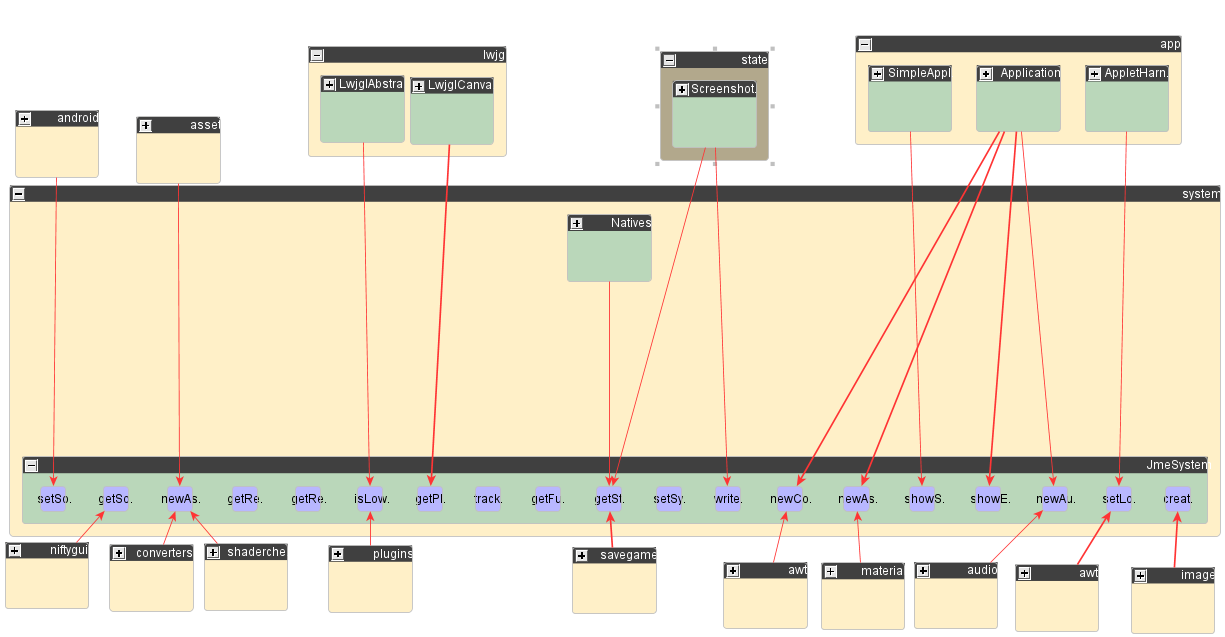
\includegraphics[width=1.3\textwidth]{figures/jme-system-deps.png}
\caption{The incoming dependencies of the JmeSystem. It is clear that these dependencies can be split up into smaller groups.}
\label{fig:system-incoming}
\end{figure}

\begin{figure}
\begin{subfigure}[b]{0.6\textwidth}
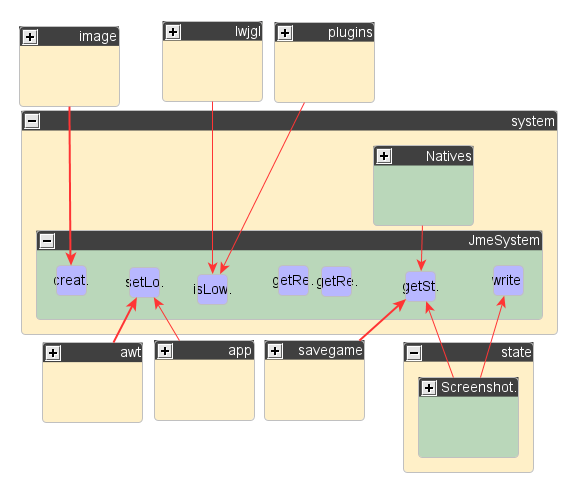
\includegraphics[width=\textwidth]{figures/jme-system-io-part.png}
\caption{This subsystem's main focus is IO, as the lowPermissions state is mostly related to which IO operations are allowed.}
\label{fig:system-io-incoming}
\end{subfigure}
~
\begin{subfigure}[b]{0.4\textwidth}
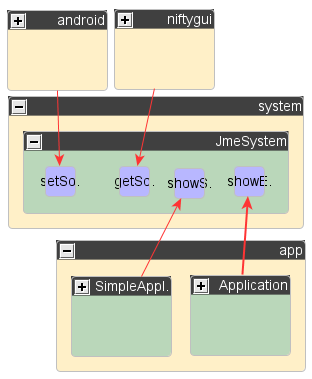
\includegraphics[width=\textwidth]{figures/jme-system-dialog-part.png}
\caption{The incoming dependencies of a sub part of JmeSystem, which we believe has the responsibility of dealing with Dialogs.}
\label{fig:system-dialog-incoming}
\end{subfigure}

\begin{subfigure}[b]{0.6\textwidth}
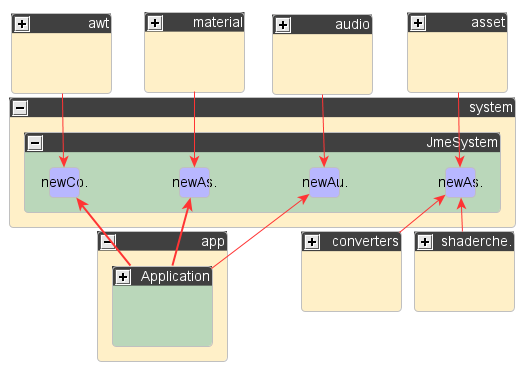
\includegraphics[width=\textwidth]{figures/jme-system-factory-part.png}
\caption{This subsystem's main focus is creating new instances of certain sytem related classes.}
\label{fig:system-factory-incoming}
\end{subfigure}
~
\begin{subfigure}[b]{0.4\textwidth}
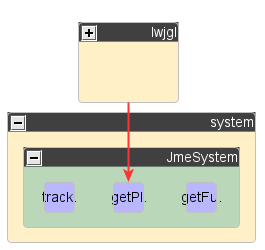
\includegraphics[width=\textwidth]{figures/jme-system-general-part.png}
\caption{The responsibility of this subsystem is handling system related state like a name and platform.}
\label{fig:system-state-incoming}
\end{subfigure}

\caption{The decomposition of JmeSystemDelegate into 4 delegates. The maximum afferent coupling for a single delegate is reduced to 9.}
\label{fig:system-decomposition}
\end{figure}


% \newpage
\section{Testsuite}
\label{sec:testsuite}
The jmonkey unit test suite is very limited.
It consists of a total of 12 unit tests and covers only 1.2\% of the jmonkey core source code.
However, none of the classes we were planning to refactor were covered.
This makes it even harder to change the JmeSystem or its delegates without breaking other code,
as there is no way of checking to what extend the change altered the behaviour.

We have written 86 test cases in total for the classes JmeSystem, JmeSystemDelegate, JmeDesktopSystem and JmeAndroidSystem.
Together with the 12 testcases that already existed, the testsuite has 98 tests (see Figure~\ref{fig:num-tests}).
This figure shows that we have a single test case with an error.
We did that on purpose, as it exposes a bug in the JmeSystemDelegate, 
where an execution branch can never be visited (equals check of a lowercase string and "PowerPC", see Figure~\ref{fig:bug}).

The testsuite is pretty extensive with an instruction coverage well in the 80\% for the classes under test (see Figures~\ref{fig:cov-core},~\ref{fig:cov-desktop}~and~\ref{fig:cov-android}).
Only JmeDesktopSystem was not covered properly at only 71\%. 
This was due to some missing classes in our project (the Jogl classes),
making it impossible to fully test the class. 
However, those non-covered parts (newContextJogl) are actually almost duplicates (supported by incode code duplicate findings) of pieces that are covered (newContextLwjgl).
So we are still confident that our testsuite suffices for the refactorings we want to make.


\begin{figure}[!hb]
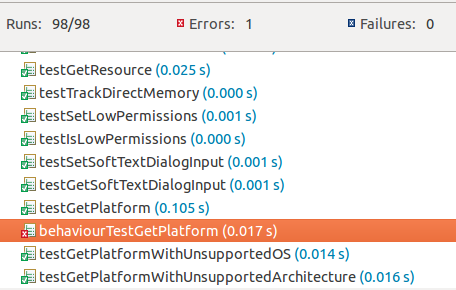
\includegraphics[width=\textwidth]{figures/86-new-tests.png}
\caption{a run of the test suite. Showing 98 testcases and a single failure (indicating the bug of Figure~\ref{fig:bug})}
\label{fig:num-tests}
\end{figure}

\begin{figure}[!hb]
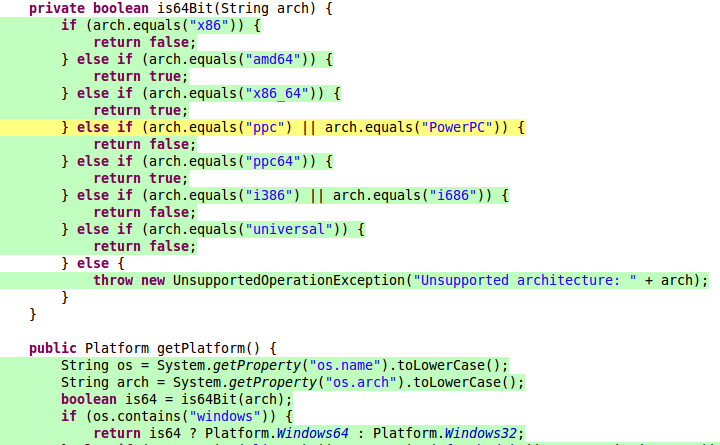
\includegraphics[width=\textwidth]{figures/bug-in-delegate.png}
\caption{The coverage indicates that the branch on matching "PowerPC" is not covered. The only call to is64 (shown at the bottom of this figure) actually only passes lowercased strings.}
\label{fig:bug}
\end{figure}

\begin{figure}[!hb]
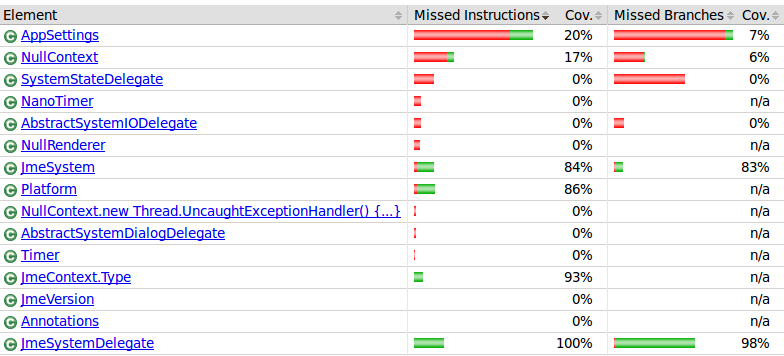
\includegraphics[width=\textwidth]{figures/test-coverage-core.png}
\caption{Test coverage for the com.jme3.system package in the src/core folder. We made testsuites for JmeSystem and JmeSystemDelegate.}
\label{fig:cov-core}
\end{figure}

\begin{figure}[!hb]
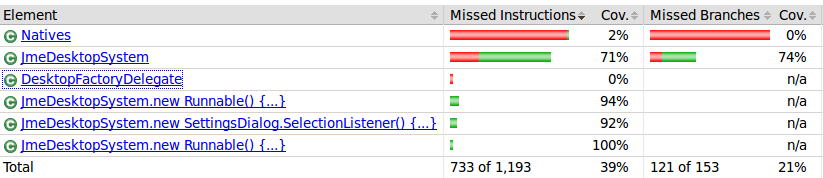
\includegraphics[width=\textwidth]{figures/test-coverage-desktop.png}
\caption{Test coverage for the com.jme3.system package in the src/desktop folder. We made a testsuite for JmeDesktopSystem.}
\label{fig:cov-desktop}
\end{figure}

\begin{figure}
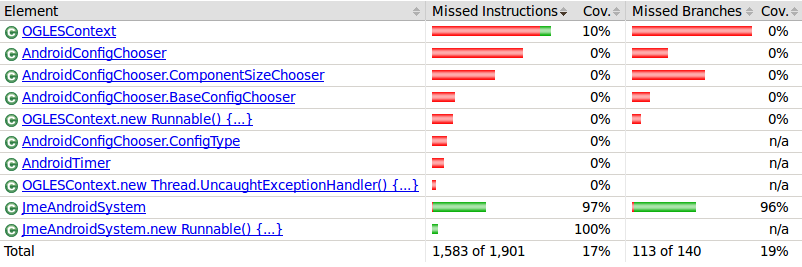
\includegraphics[width=\textwidth]{figures/test-coverage-android.png}
\caption{Test coverage for the com.jme3.system.android package in the src/android folder. We made a testsuite for JmeAndroidSystem.}
\label{fig:cov-android}
\end{figure}

\end{document}
